\documentclass[aspectratio=169,10pt]{beamer}
\usetheme{Madrid}
\usecolortheme{seahorse}

\usepackage[utf8]{inputenc}
\usepackage{amsmath}
\usepackage{amssymb}
\usepackage{amsfonts}
\usepackage{graphicx}
\usepackage{listings}
\usepackage{xcolor}
\usepackage{tikz}
\usepackage{cite}

\graphicspath{{figures/}}

% Code style for Python
\lstset{
  basicstyle=\ttfamily\scriptsize,
  keywordstyle=\color{blue},
  commentstyle=\color{green!50!black}\itshape,
  stringstyle=\color{red},
  showstringspaces=false,
  breaklines=true,
  frame=single,
  numbers=left,
  numberstyle=\tiny,
  language=Python
}

\setbeamertemplate{footline}[frame number]

\title{Metric \& Normed Spaces}
\subtitle{Pathak -- Chapter 1b: Spaces, Operators, Duality and Compactness}
\author{Nonlinear Analysis and Fixed Point Theory}
\date{2018}

\begin{document}

\frame{\titlepage}

% ==============================================================================
% SECTION 1: Hilbert Spaces and Overview
% ==============================================================================

\section{1.2: Hilbert Spaces}

\begin{frame}{Hilbert Spaces}
  \begin{definition}[Hilbert Space]
    A \textbf{Hilbert space} $\mathcal{H}$ is an inner product space $(\mathcal{H}, \langle \cdot, \cdot \rangle)$ such that the induced norm $\|x\| = \sqrt{\langle x, x \rangle}$ is complete (every Cauchy sequence converges).
  \end{definition}

  \vspace{0.3cm}
  \textbf{Key Properties:}
  \begin{itemize}
    \item Complete inner product space with norm $\|x\| = \sqrt{\langle x, x \rangle}$
    \item Parallelogram law holds: $\|x+y\|^2 + \|x-y\|^2 = 2(\|x\|^2 + \|y\|^2)$
    \item Banach space with additional structure
  \end{itemize}

  \vspace{0.3cm}
  \textbf{Examples:}
  \begin{itemize}
    \item $\mathbb{R}$ and $\mathbb{C}$ with usual inner products
    \item $\ell^2 = \left\{ x = (x_i) : \sum_{i=1}^{\infty} |x_i|^2 < \infty \right\}$ with $\langle x, y \rangle = \sum_{i=1}^{\infty} x_i y_i$
    \item $L^2[a,b]$ with $\langle f, g \rangle = \int_a^b f(t)g(t) dt$
    \item $C[a,b]$ with an appropriate inner product (normed but not Hilbert in the sup norm)
  \end{itemize}
\end{frame}

\begin{frame}{When is $\ell_p$ a Hilbert Space?}
  \textbf{Example 1.24:} For $p \neq 2$, $\ell_p$ is NOT a Hilbert space.

  \vspace{0.3cm}
  \textbf{Counterexample with $p = 3$:}
  Let $x = (1, -1, 1, 0, \ldots)$ and $y = (-1, 1, 1, 0, \ldots)$. Then:
  \begin{align*}
    \|x\| &= (1 + 1 + 1)^{1/3} = 3^{1/3} \\
    \|y\| &= (1 + 1 + 1)^{1/3} = 3^{1/3} \\
    \|x + y\| &= (2)^{1/3}, \quad \|x - y\| &= (2 + 2)^{1/3} = 4^{1/3}
  \end{align*}

  \vspace{0.2cm}
  \textbf{Check parallelogram law:}
  $$\|x+y\|^2 + \|x-y\|^2 = 2^{2/3} + 4^{2/3} \neq 2 \cdot 2 \cdot 3^{2/3}$$

  \vspace{0.2cm}
  The parallelogram law \textbf{fails} for $p \neq 2$, so $\ell_p$ is not Hilbert.

  \vspace{0.2cm}
  \boxed{\text{Only } \ell^2 \text{ is a Hilbert space among } \{\ell_p : p \geq 1\}}
\end{frame}

% ==============================================================================
% SECTION 2: Bounded Linear Operators
% ==============================================================================

\section{1.3: Bounded Linear Operators}

\begin{frame}{Linear Operators and Functionals}
  \begin{definition}[Linear Operator]
    Let $X, Y$ be vector spaces. An operator $A : X \to Y$ is \textbf{linear} if:
    \begin{enumerate}
      \item \textit{Additive}: $A(x + y) = Ax + Ay$ for all $x, y \in X$
      \item \textit{Homogeneous}: $A(\alpha x) = \alpha A(x)$ for all $x \in X, \alpha \in \mathbb{K}$
    \end{enumerate}
    Equivalently: $A(\alpha x + \beta y) = \alpha A(x) + \beta A(y)$ for all $x, y \in X, \alpha, \beta \in \mathbb{K}$.
  \end{definition}

  \vspace{0.3cm}
  \textbf{Linear Functional:} If $Y = \mathbb{K}$, then $A$ is called a \textbf{linear functional}.

  \vspace{0.3cm}
  \textbf{Note:} A linear operator \textbf{need not be continuous} in infinite-dimensional spaces!

  \vspace{0.3cm}
  \textbf{Key Operators Example:}
  \begin{itemize}
    \item $Ax = \sum_{i=1}^{n} a_i x_i$ on $\mathbb{R}^n$ (linear functional)
    \item $Ax = (x_2/2, x_3/4, \ldots, x_n/n^2, \ldots)$ on $\ell_2$ (linear operator)
    \item $[Ax](s) = \int_0^s x(t)y(t) dt$ on $L_2[0, 2\pi]$ (linear functional)
  \end{itemize}
\end{frame}

\begin{frame}{Bounded Linear Operators}
  \begin{definition}[Bounded Linear Operator]
    A linear operator $A : X \to Y$ between normed spaces is \textbf{bounded} if there exists $M > 0$ such that:
    $$\|Ax\| \leq M\|x\| \quad \text{for all } x \in X$$
  \end{definition}

  \vspace{0.3cm}
  \textbf{Important Terminology:}
  \begin{itemize}
    \item \textit{Bounded} does NOT mean image is bounded
    \item Rather: bounded sets map to bounded sets
    \item Equivalently: linear operator is bounded iff continuous
  \end{itemize}

  \vspace{0.3cm}
  \textbf{Operator Norm:}
  $$\|A\|_B = \inf\{M : \|Ax\| \leq M\|x\|, \forall x \in X\} = \sup_{\|x\| \leq 1} \|Ax\| = \sup_{x \neq 0} \frac{\|Ax\|}{\|x\|}$$

  \vspace{0.3cm}
  \begin{theorem}[Theorem 1.13]
    For normed spaces $X, Y$: A linear operator $A : X \to Y$ is bounded if and only if it is continuous.
  \end{theorem}
\end{frame}

\begin{frame}{Example: Unbounded Linear Operator}
  \textbf{Example 1.26:} Not all linear operators are bounded!

  \vspace{0.3cm}
  Let $c_{00}$ = space of finitely nonzero sequences with supremum norm $\|\cdot\|_\infty$.

  \vspace{0.3cm}
  Define $A : c_{00} \to \mathbb{R}$ by:
  $$Ax = \sum_{i=1}^{n} i x_i \quad \text{for } x = (x_1, \ldots, x_n, 0, 0, \ldots)$$

  \vspace{0.3cm}
  \textbf{Linear?} Yes. $A(\alpha x + \beta y) = \alpha A(x) + \beta A(y)$.

  \vspace{0.3cm}
  \textbf{Unbounded?} Consider $x_n = (1, 1, \ldots, 1, 0, 0, \ldots)$ ($n$ ones):
  \begin{align*}
    \|x_n\|_\infty &= 1 \\
    Ax_n &= 1 + 2 + \cdots + n = \frac{n(n+1)}{2} \to \infty
  \end{align*}

  \vspace{0.2cm}
  \boxed{\text{No } M \text{ exists such that } |Ax_n| \leq M \cdot 1 \text{ for all } n}

  \vspace{0.3cm}
  \textcolor{red}{\textbf{Key Lesson:}} Even simple looking operators can be unbounded on infinite-dimensional spaces!
\end{frame}

\begin{frame}{The Space $B(X, Y)$ of Bounded Linear Operators}
  \begin{definition}
    Let $B(X, Y)$ denote the family of all bounded linear operators from $X$ to $Y$.
  \end{definition}

  \vspace{0.3cm}
  \textbf{Vector Space Structure:}
  \begin{itemize}
    \item $(A_1 + A_2)(x) = A_1(x) + A_2(x)$
    \item $(\alpha A)(x) = \alpha A(x)$
    \item Forms a normed space with $\|A\|_B = \sup_{\|x\| \leq 1} \|Ax\|$
  \end{itemize}

  \vspace{0.3cm}
  \begin{theorem}[Theorem 1.14 --- Uniform Boundedness Principle]
    If $X$ is a Banach space, $Y$ is a normed space, and $\{A_i\}_{i \in I}$ is a family of bounded operators such that $\{A_i x : i \in I\}$ is bounded for each $x \in X$, then $\{A_i\}$ is uniformly bounded: $\sup_i \|A_i\|_B < \infty$.
  \end{theorem}

  \vspace{0.3cm}
  \textbf{Consequence:} If $Y$ is also Banach, then $B(X, Y)$ is a Banach space.

  \vspace{0.2cm}
  \begin{center}
    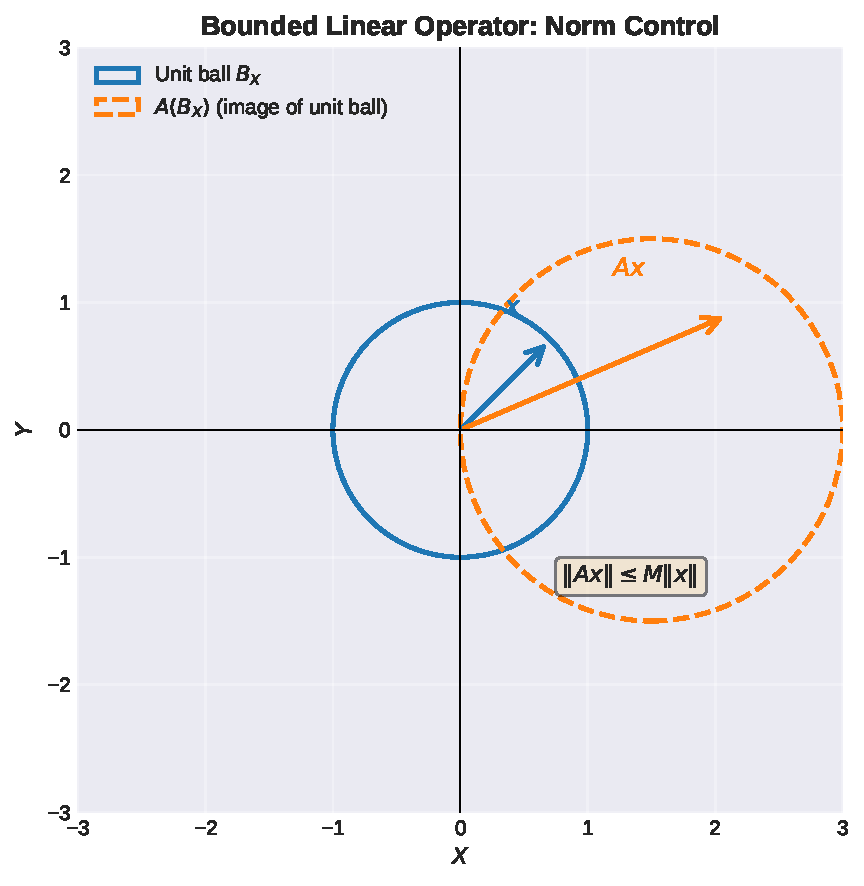
\includegraphics[width=0.6\linewidth]{operator_norm.pdf}
  \end{center}
\end{frame}

\begin{frame}{Convergence of Operators}
  Let $(X, \|\cdot\|_X)$ and $(Y, \|\cdot\|_Y)$ be normed spaces, and $\{T_n\} \subseteq B(X,Y)$.

  \vspace{0.2cm}
  \begin{definition}[Three Types of Operator Convergence]
    \begin{enumerate}
      \item \textbf{Uniform convergence:} $T_n \to T$ uniformly if $\|T_n - T\|_B \to 0$
      \vspace{0.1cm}

      \item \textbf{Strong convergence:} $T_n \to T$ strongly if $\|T_n x - Tx\|_Y \to 0$ for each $x \in X$
      \vspace{0.1cm}

      \item \textbf{Weak convergence:} $T_n \to T$ weakly if $|f(T_n x) - f(Tx)| \to 0$ for all $x \in X, f \in Y^*$
    \end{enumerate}
  \end{definition}

  \vspace{0.3cm}
  \begin{theorem}[Theorem 1.15]
    If $\{A_n\}$ is a sequence of bounded operators with $A_n x \to Ax$ for each $x \in X$ (strong convergence), then $A \in B(X, Y)$ and $\|A\|_B \leq \liminf_{n \to \infty} \|A_n\|_B$.
  \end{theorem}

  \vspace{0.2cm}
  \begin{center}
    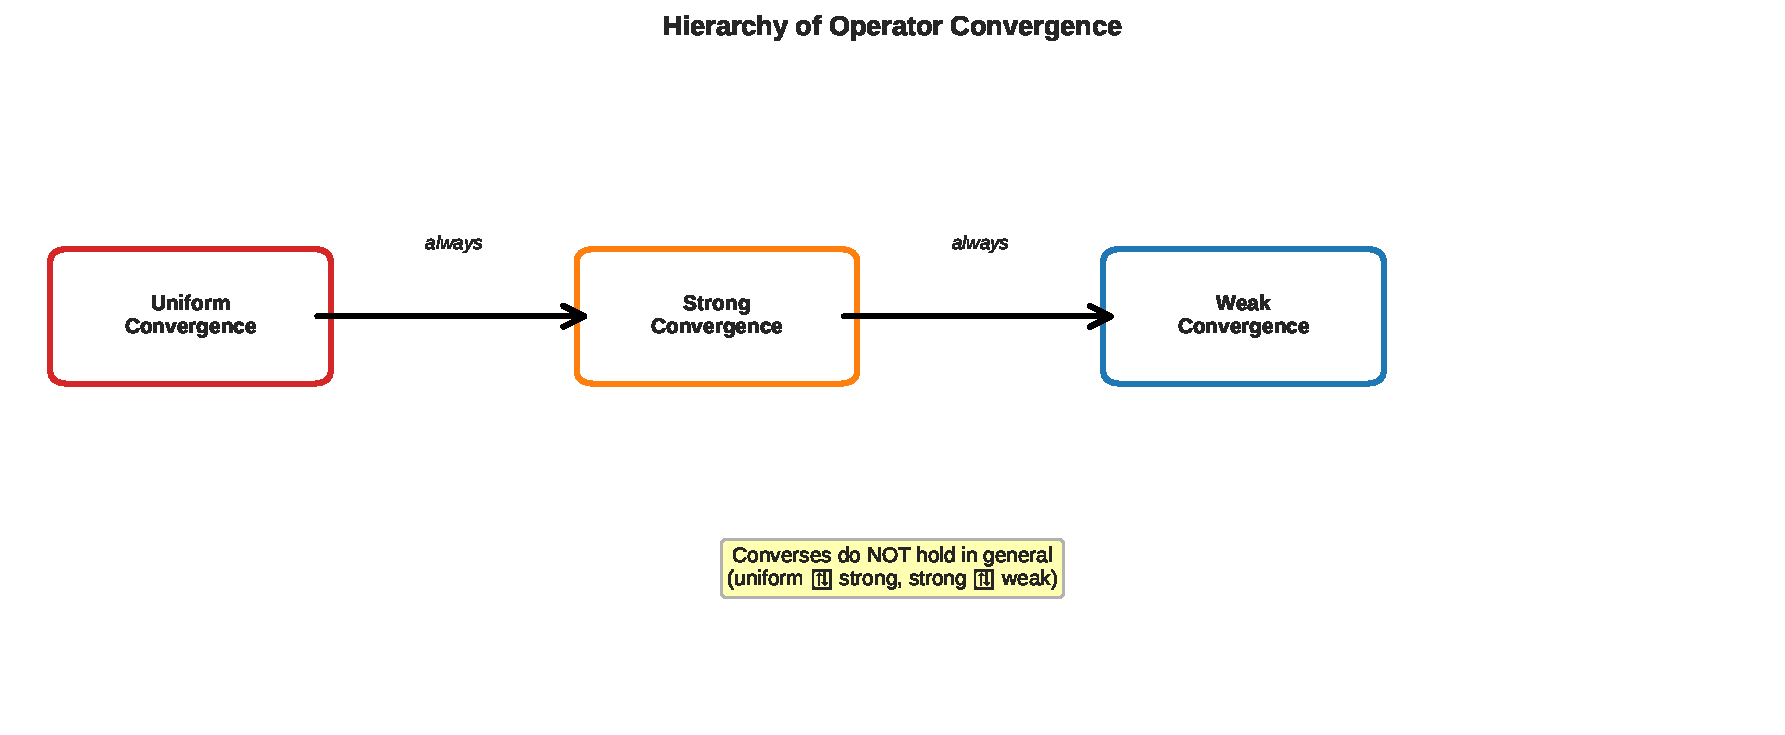
\includegraphics[width=0.65\linewidth]{convergence_hierarchy.pdf}
  \end{center}
\end{frame}

\begin{frame}[fragile]{Code: Operator Norm in Python}
  \begin{lstlisting}[language=Python]
import numpy as np
from scipy.linalg import norm

# Define a linear operator (matrix)
A = np.array([[1, 2], [3, 4]])

# Operator norm ||A||_B = max ||Ax|| / ||x||
# For matrices, this is the largest singular value
operator_norm = np.linalg.norm(A, ord=2)  # spectral norm
print(f"Operator norm: {operator_norm:.4f}")

# Verify: ||Ax|| <= operator_norm * ||x||
x = np.array([1, 1])
x_norm = np.linalg.norm(x)
Ax = A @ x
Ax_norm = np.linalg.norm(Ax)
ratio = Ax_norm / x_norm

print(f"||x|| = {x_norm:.4f}")
print(f"||Ax|| = {Ax_norm:.4f}")
print(f"||Ax|| / ||x|| = {ratio:.4f} <= {operator_norm:.4f}")
  \end{lstlisting}
\end{frame}

\begin{frame}{Banach Algebra}
  \begin{definition}[Algebra over a Field]
    A linear space $\mathcal{A}$ over field $\mathbb{K}$ with multiplication $x \cdot y \in \mathcal{A}$ is an \textbf{algebra} if:
    \begin{enumerate}
      \item $(xy)z = x(yz)$ (associativity)
      \item $x(y + z) = xy + xz$ (distributivity)
      \item $(x + y)z = xz + yz$ (distributivity)
      \item $\alpha(xy) = (\alpha x)y = x(\alpha y)$ (scalar compatibility)
    \end{enumerate}
  \end{definition}

  \vspace{0.3cm}
  \begin{definition}[Normed Algebra / Banach Algebra]
    An algebra $\mathcal{A}$ is a \textbf{normed algebra} if it is a normed space with:
    $$\|xy\| \leq \|x\| \|y\| \quad \text{for all } x, y \in \mathcal{A}$$

    A \textbf{Banach algebra} is a complete normed algebra.
  \end{definition}

  \vspace{0.3cm}
  \textbf{Examples:}
  \begin{itemize}
    \item $\mathbb{R}$ and $\mathbb{C}$ are Banach algebras
    \item $C[a,b]$ with pointwise multiplication: commutative Banach algebra
    \item $B(X)$ of bounded operators on Banach space $X$: non-commutative Banach algebra
  \end{itemize}
\end{frame}

% ==============================================================================
% SECTION 3: The Hahn-Banach Theorem
% ==============================================================================

\section{1.4: The Hahn-Banach Theorem}

\begin{frame}{The Hahn-Banach Theorem (Real Case)}
  One of the most important theorems in functional analysis.

  \vspace{0.3cm}
  \begin{definition}[Sublinear Functional]
    A functional $p : X \to \mathbb{R}$ is \textbf{sublinear} if:
    \begin{enumerate}
      \item $p(x + y) \leq p(x) + p(y)$ for all $x, y \in X$ (subadditivity)
      \item $p(\alpha x) = \alpha p(x)$ for all $x \in X, \alpha \geq 0$ (positive homogeneity)
    \end{enumerate}
  \end{definition}

  \vspace{0.3cm}
  \begin{theorem}[Theorem 1.16 --- Hahn-Banach, Real Case]
    Let $X$ be a real linear space, $Y$ a subspace, $p$ a sublinear functional on $X$, and $f$ a linear functional on $Y$ with $f(x) \leq p(x)$ for all $x \in Y$.

    Then there exists a linear extension $F : X \to \mathbb{R}$ such that:
    \begin{itemize}
      \item $F(x) = f(x)$ for all $x \in Y$
      \item $F(x) \leq p(x)$ for all $x \in X$
    \end{itemize}
  \end{theorem}

  \vspace{0.2cm}
  \textbf{Intuition:} Can always extend functionals preserving bounds.
\end{frame}

\begin{frame}{Hahn-Banach for Normed Spaces}
  \begin{theorem}[Theorem 1.17 --- Hahn-Banach, Normed Case]
    Let $X$ be a real normed space, $Y$ a subspace of $X$, and $f \in Y^*$ a bounded linear functional on $Y$.

    Then there exists $F \in X^*$ such that:
    \begin{itemize}
      \item $F(x) = f(x)$ for all $x \in Y$
      \item $\|F\|_* = \|f\|_*$
    \end{itemize}

    Every bounded functional on a subspace extends to the whole space with preservation of norm.
  \end{theorem}

  \vspace{0.3cm}
  \textbf{Immediate Corollaries:}

  \begin{corollary}[Corollary 1.2]
    For any nonzero $x \in X$, there exists $f \in X^*$ with $f(x) = \|x\|$ and $\|f\|_* = 1$.
  \end{corollary}

  \begin{corollary}[Corollary 1.3]
    For any nonzero $x \in X$, there exists $f \in X^*$ with $f(x) = \|x\|$ and $\|f\|_* = 1$.
  \end{corollary}

  \vspace{0.2cm}
  \textbf{Consequence:} Enough bounded functionals to separate points!
\end{frame}

\begin{frame}{Geometric Forms: Hyperplanes}
  \begin{definition}[Hyperplane]
    A subset $H$ of linear space $X$ is a \textbf{hyperplane} if there exists a nonzero linear functional $f$ and scalar $\alpha$ such that:
    $$H = \{x \in X : f(x) = \alpha\}$$
  \end{definition}

  \vspace{0.3cm}
  \textbf{Example 1.28:} In $\mathbb{R}$, let $f(x) = \frac{3}{7}x$ and $\alpha = 4$.
  $$H = \left\{x : \frac{3}{7}x = 4\right\} = \left\{\frac{28}{3}\right\}$$
  This is a ``hyperplane'' (single point) in $\mathbb{R}$.

  \vspace{0.3cm}
  \begin{theorem}[Theorem 1.18 --- Separation Theorem]
    Let $M$ be a subspace of normed space $X$, $x_0 \in X$ with $d(x_0, M) = d > 0$. Then there exists a bounded linear functional $j \in X^*$ with unit norm such that:
    \begin{itemize}
      \item $j(x_0) = d$
      \item $j(x) = 0$ for all $x \in M$
    \end{itemize}
  \end{theorem}

  \vspace{0.2cm}
  \textbf{Intuition:} Can separate element from subspace with a functional.
\end{frame}

\begin{frame}{The Dual Space (Conjugate Space)}
  \begin{definition}[Dual Space]
    The \textbf{dual space} $X^*$ of normed space $X$ is the space $B(X, \mathbb{K})$ of all bounded linear functionals on $X$.
  \end{definition}

  \vspace{0.3cm}
  \textbf{Norm on } $X^*$:
  $$\|f\|_* = \sup_{x \neq 0} \frac{|f(x)|}{\|x\|} = \sup_{\|x\| \leq 1} |f(x)|$$

  \vspace{0.3cm}
  \textbf{Key Fact:} If $X$ is Banach, then $X^*$ is also Banach.

  \vspace{0.3cm}
  \textbf{Examples of Dual Spaces:}
  \begin{enumerate}
    \item $(\mathbb{R}^n)^* = \mathbb{R}^n$ (isometric isomorphism)
    \item $(\ell_p)^* = \ell_q$ where $\frac{1}{p} + \frac{1}{q} = 1$
    \item $(c_0)^* = \ell_1$ (sequences summable to 0 pair with $\ell_1$)
    \item $(L_p(\Omega))^* = L_q(\Omega)$ where $\frac{1}{p} + \frac{1}{q} = 1$
    \item $(C(\Omega))^* = M(\Omega)$ (space of Radon measures)
  \end{enumerate}

  \begin{center}
    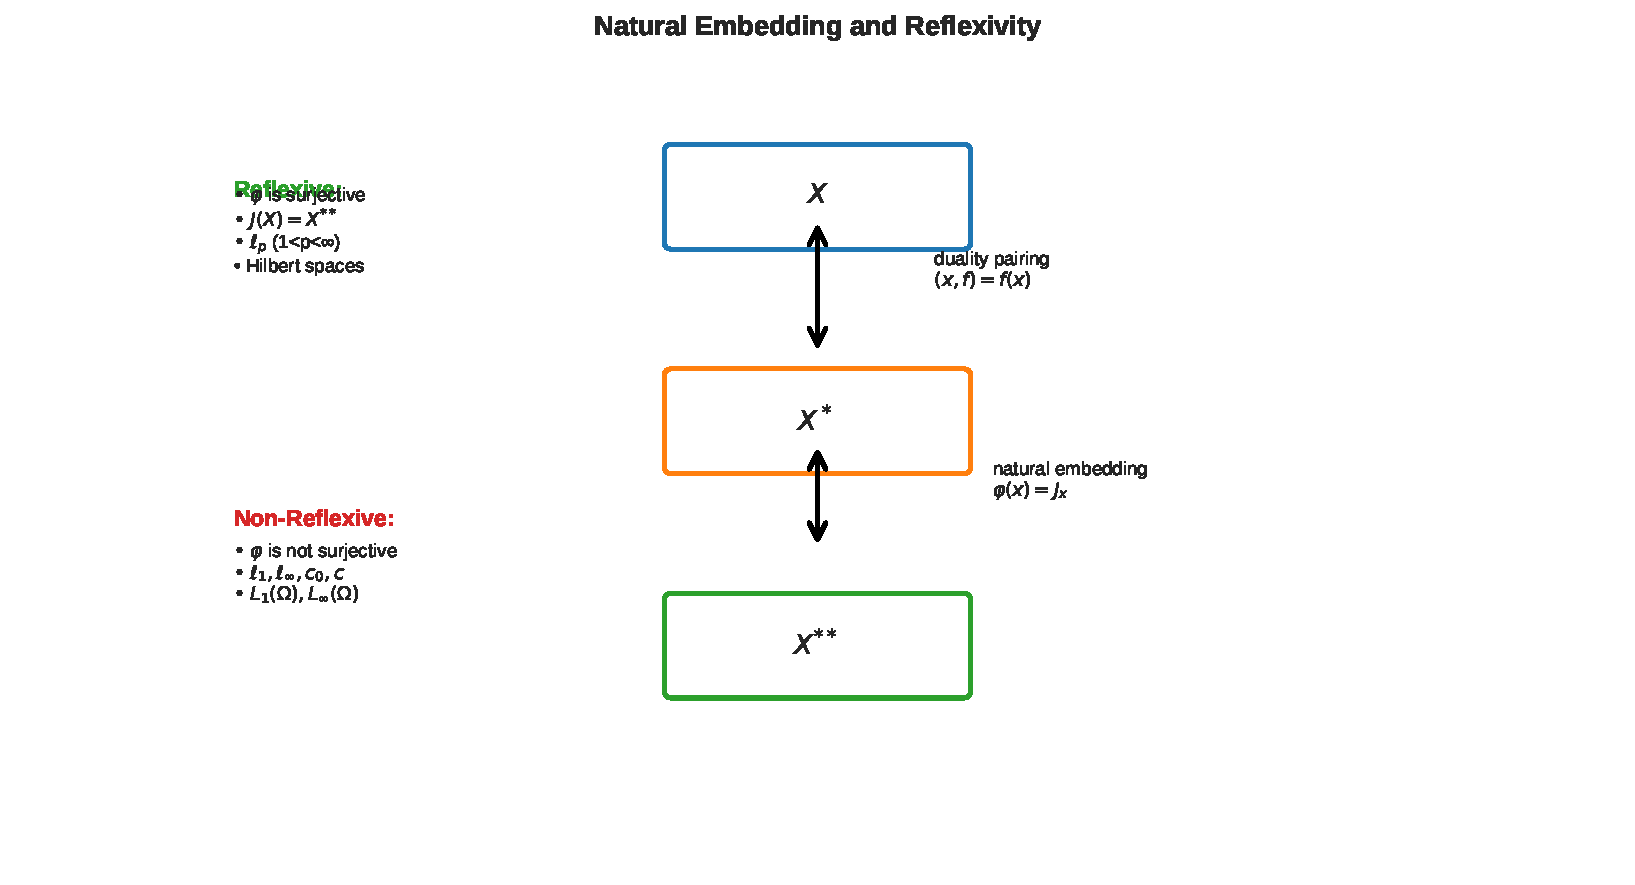
\includegraphics[width=0.65\linewidth]{reflexivity_diagram.pdf}
  \end{center}
\end{frame}

\begin{frame}{Natural Embedding and Reflexivity}
  \begin{definition}[Natural Embedding Mapping]
    For normed space $X$, define $\varphi : X \to X^{**}$ by:
    $$\varphi(x)(f) = f(x) \quad \text{for all } x \in X, f \in X^*$$
    This is called the \textbf{natural embedding mapping}.
  \end{definition}

  \vspace{0.3cm}
  \textbf{Properties of } $\varphi$:
  \begin{itemize}
    \item \textbf{Linear}: $\varphi(\alpha x + \beta y) = \alpha \varphi(x) + \beta \varphi(y)$
    \item \textbf{Isometric}: $\|\varphi(x)\| = \|x\|$ for all $x \in X$
  \end{itemize}

  \vspace{0.3cm}
  \begin{definition}[Reflexive Space]
    A Banach space $X$ is \textbf{reflexive} if the natural embedding $\varphi : X \to X^{**}$ is surjective (i.e., $\varphi(X) = X^{**}$).
  \end{definition}

  \vspace{0.3cm}
  \textbf{Examples:}
  \begin{itemize}
    \item Reflexive: $\ell^p$ for $1 < p < \infty$, Hilbert spaces, finite-dimensional spaces
    \item Non-reflexive: $\ell^1$, $c_0$, $c$, $L_1(\Omega)$, $C(\Omega)$
  \end{itemize}
\end{frame}

\begin{frame}{Key Theorems on Reflexive Spaces}
  \begin{theorem}[Theorem 1.21 --- James' Theorem]
    If $X$ is a reflexive Banach space, then every $f \in X^*$ attains its norm on the unit ball $\mathbb{B}_X$.
  \end{theorem}

  \vspace{0.3cm}
  \begin{theorem}[Theorem 1.22]
    A Banach space $X$ is reflexive if and only if every $f \in X^*$ attains its norm on the unit ball $\mathbb{B}_X$.
  \end{theorem}

  \vspace{0.3cm}
  \begin{theorem}[Theorem 1.23 --- Riesz Representation Theorem]
    Let $(\mathcal{H}, \langle \cdot, \cdot \rangle)$ be a Hilbert space and $f \in \mathcal{H}^*$. Then there exists a unique $y \in \mathcal{H}$ such that:
    $$f(x) = \langle x, y \rangle$$
    Moreover, $\|f\|_* = \|y\|$.
  \end{theorem}

  \vspace{0.3cm}
  \textbf{Consequence:} All Hilbert spaces are reflexive.

  \vspace{0.2cm}
  \textbf{Remark 1.8:} In Hilbert spaces, $\mathcal{H}^* = \mathcal{H}$ (in the sense of isometric isomorphism).
\end{frame}

\begin{frame}{Multilinear Mappings}
  \begin{definition}[Multilinear Mapping]
    A mapping $A : X_1 \times X_2 \times \cdots \times X_n \to Y$ is \textbf{multilinear} if it is linear in each variable separately.
  \end{definition}

  \vspace{0.3cm}
  \begin{definition}[Bounded Multilinear Mapping]
    A multilinear mapping $A$ is \textbf{bounded} if there exists $\mu > 0$ such that:
    $$\|A(x_1, x_2, \ldots, x_n)\| \leq \mu \|x_1\| \|x_2\| \cdots \|x_n\|$$
  \end{definition}

  \vspace{0.3cm}
  \begin{theorem}[Theorem 1.20]
    There is an isometric isomorphism between $\mathcal{L}(X_1, X_2; Y)$ and $\mathcal{L}(X_1, \mathcal{L}(X_2, Y))$.
  \end{theorem}

  \vspace{0.3cm}
  \textbf{Consequence:} Multilinear maps reduce to iterates of linear maps:
  $$\mathcal{L}(X_1, X_2, X_3; Y) \cong \mathcal{L}(X_1, \mathcal{L}(X_2, \mathcal{L}(X_3, Y)))$$
\end{frame}

\begin{frame}{Weak Topologies}
  \begin{definition}[Weak Topology on $X$]
    The \textbf{weak topology} $\sigma(X, X^*)$ on normed space $X$ is the weakest topology making all functionals $f \in X^*$ continuous.
  \end{definition}

  \vspace{0.3cm}
  \textbf{Weak Neighborhoods:} A set $G \subseteq X$ is open in weak topology if for each $x \in G$, there exist $f_1, \ldots, f_n \in X^*$ and $\epsilon_1, \ldots, \epsilon_n > 0$ such that:
  $$\{y \in X : |f_i(x) - f_i(y)| < \epsilon_i, i = 1, \ldots, n\} \subseteq G$$

  \vspace{0.3cm}
  \begin{definition}[Weak Convergence]
    A sequence $\{x_n\}$ \textbf{weakly converges} to $x$ (written $x_n \rightharpoonup x$) if:
    $$f(x_n) \to f(x) \quad \text{for all } f \in X^*$$
  \end{definition}

  \vspace{0.3cm}
  \begin{observation}
    \begin{itemize}
      \item Weak topology is weaker than norm topology (fewer open sets)
      \item Strong convergence implies weak convergence (not conversely!)
      \item In finite dimensions: weak = strong convergence
      \item Hilbert/reflexive spaces: weak* topology = weak topology on $X^*$
    \end{itemize}
  \end{observation}

  \begin{center}
    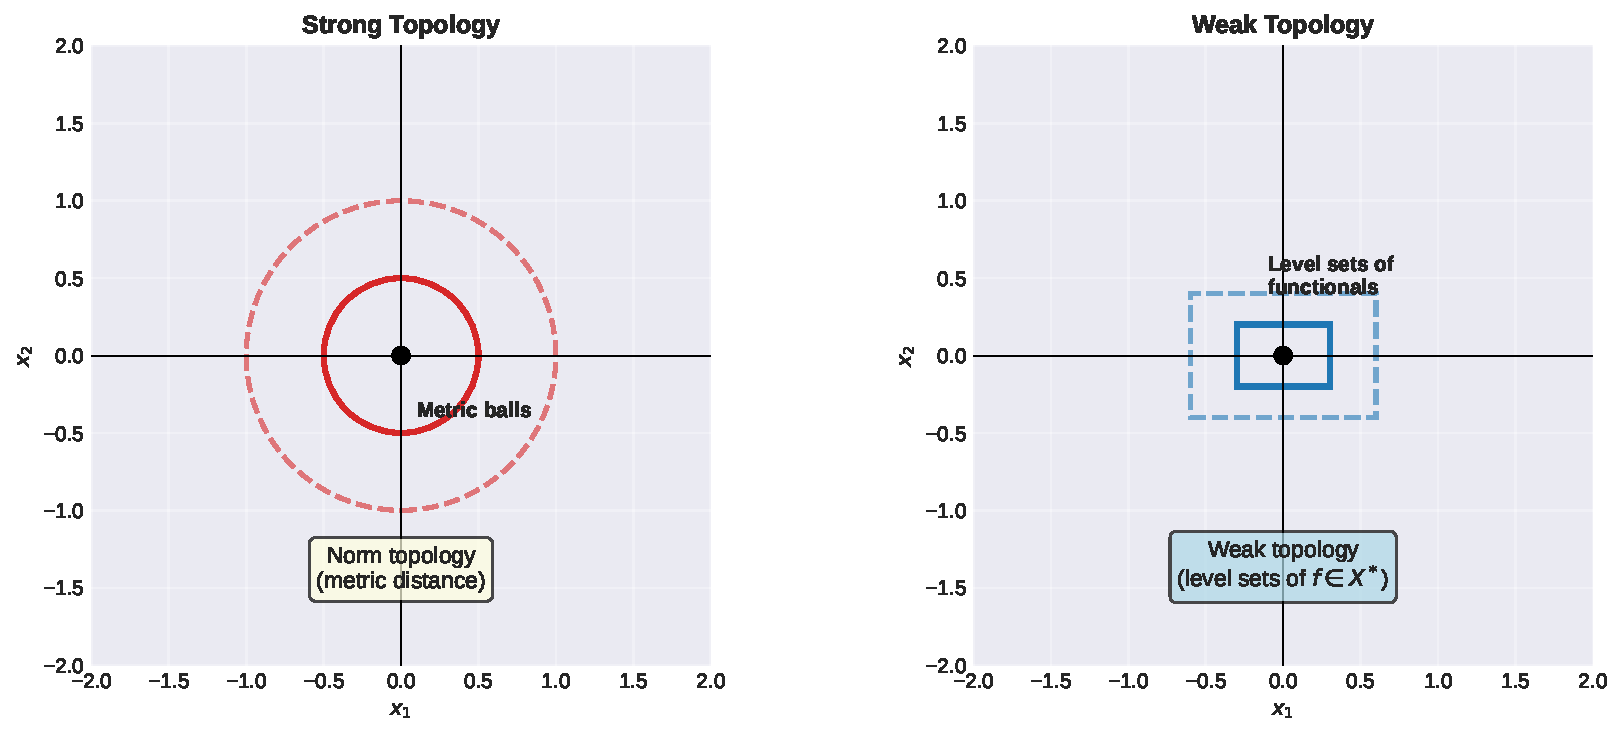
\includegraphics[width=0.65\linewidth]{topology_comparison.pdf}
  \end{center}
\end{frame}

\begin{frame}{Properties of Weakly Convergent Sequences}
  \begin{proposition}[Proposition 1.9]
    The weak limit is unique.
  \end{proposition}

  \vspace{0.2cm}
  \begin{proposition}[Proposition 1.10]
    If $x_n \to x$ strongly, then $x_n \rightharpoonup x$ weakly.
  \end{proposition}

  \vspace{0.3cm}
  \textbf{Example 1.31:} Converse fails in $\ell_2$. Let $e_n = (0, \ldots, 1, 0, \ldots)$ (1 in $n$-th position).
  \begin{align*}
    \|e_n\|_2 &= 1 \quad \text{(NOT converging to 0 in norm)} \\
    \langle e_n, y \rangle &= y_n \to 0 \quad \text{(converges weakly to 0 for any } y \in \ell_2\text{)}
  \end{align*}

  \vspace{0.2cm}
  $\Rightarrow$ Weak convergence does NOT imply strong convergence!

  \vspace{0.3cm}
  \begin{proposition}[Proposition 1.11 --- Weak convergence in $\ell_p$]
    For $1 < p < \infty$, $x_n = (x_n^{(i)}) \rightharpoonup x = (x_i)$ in $\ell_p$ iff:
    \begin{enumerate}
      \item $\{x_n\}$ is bounded: $\sup_n \|x_n\|_p < \infty$
      \item Coordinatewise convergence: $x_n^{(i)} \to x_i$ for all $i$
    \end{enumerate}
  \end{proposition}
\end{frame}

\begin{frame}{Weak* Topology and Schur Property}
  \begin{definition}[Weak* Topology on $X^*$]
    The \textbf{weak* topology} $\sigma(X^*, X)$ is the weakest topology making all evaluation functionals $e_x(f) = f(x)$ continuous.
  \end{definition}

  \vspace{0.3cm}
  \textbf{Weak* Convergence:} $f_n \xrightarrow{w^*} f$ in $X^*$ iff $f_n(x) \to f(x)$ for all $x \in X$.

  \vspace{0.3cm}
  \begin{definition}[Schur Property]
    A normed space $X$ has the \textbf{Schur property} if every weakly convergent sequence in $X$ converges in norm.
  \end{definition}

  \vspace{0.3cm}
  \begin{lemma}[Lemma 1.1 --- Schur's Lemma]
    $\ell^1$ has the Schur property: if $x^n \rightharpoonup 0$ in $\ell_1$, then $\|x^n\|_1 \to 0$.
  \end{lemma}

  \vspace{0.3cm}
  \textbf{Crucial Relationships:}
  \begin{itemize}
    \item $(c_0)^* = \ell_1$ and $(\ell_1)^* = \ell_\infty$
    \item $c^* = \ell_1$ (sequences converging to constant pair with $\ell_1$)
    \item Weak convergence in $\ell_1 \Rightarrow$ coordinatewise convergence
  \end{itemize}
\end{frame}

\begin{frame}{Convergence in the Dual Space}
  Let $X$ be a normed space and $\{f_n\} \subseteq X^*$.

  \vspace{0.2cm}
  \begin{enumerate}
    \item \textbf{Norm convergence}: $f_n \to f$ if $\|f_n - f\|_* \to 0$
    \vspace{0.1cm}

    \item \textbf{Weak convergence on } $X^*$: $f_n \rightharpoonup f$ (weak) if $(f_n - f, g) \to 0$ for all $g \in X^{**}$
    \vspace{0.1cm}

    \item \textbf{Weak* convergence on } $X^*$: $f_n \xrightarrow{w^*} f$ if $f_n(x) \to f(x)$ for all $x \in X$
  \end{enumerate}

  \vspace{0.3cm}
  \textbf{Relationships:}
  $$\text{Norm convergence} \Rightarrow \text{Weak convergence} \Rightarrow \text{Weak* convergence}$$

  \vspace{0.3cm}
  \begin{proposition}[Proposition 1.12]
    Let $C$ be a convex subset of normed space $X$. Then $C$ is weakly closed iff $C$ is norm closed.
  \end{proposition}

  \vspace{0.3cm}
  \textbf{Intuition:} For convex sets, weak and norm closure coincide!
\end{frame}

\begin{frame}[fragile]{Code: Weak Convergence Example}
  \begin{lstlisting}[language=Python]
import numpy as np

# Weak convergence in l^2:
# x_n = (0, ..., 1, 0, ...) (1 in n-th position)
# x_n weakly converges to 0 but ||x_n||_2 = 1 (no strong convergence)

def weak_convergence_l2(N=100):
    """Demonstrate weak vs strong convergence in l^2"""

    # Generate sequences
    for n in [10, 50, 100, 200]:
        # Standard basis vector e_n
        x_n = np.zeros(n)
        x_n[n-1] = 1.0  # 1 in n-th position

        # Strong norm
        strong_norm = np.linalg.norm(x_n)

        # Weak convergence test: inner product with arbitrary y
        y = np.random.randn(n)
        weak_value = np.dot(x_n, y)

        print(f"n={n:3d}: ||x_n||_2 = {strong_norm:.4f}, "
              f"<x_n, y> = {weak_value/np.linalg.norm(y):.6f}")

    print("\n||x_n|| stays at 1.0 (no strong convergence)")
    print("<x_n, y> / ||y|| -> 0 (weak convergence)")

weak_convergence_l2()
  \end{lstlisting}
\end{frame}

% ==============================================================================
% SECTION 4: Compactness
% ==============================================================================

\section{1.5: Compactness}

\begin{frame}{Compactness in Metric Spaces}
  \begin{definition}[Compact Metric Space]
    A metric space $X$ is \textbf{compact} if every open cover has a finite subcover. Equivalently, every sequence has a convergent subsequence.
  \end{definition}

  \vspace{0.3cm}
  \begin{definition}[Totally Bounded (Precompact)]
    A subset $C$ of metric space $X$ is \textbf{totally bounded} if for each $\epsilon > 0$, there exists a finite set $\{x_1, \ldots, x_n\} \subseteq X$ such that:
    $$C \subseteq \bigcup_{i=1}^{n} B(x_i, \epsilon)$$
  \end{definition}

  \vspace{0.3cm}
  \begin{proposition}[Proposition 1.15]
    For a metric space $X$, the following are equivalent:
    \begin{enumerate}
      \item $X$ is compact
      \item Every sequence has a convergent subsequence
      \item $X$ is totally bounded and complete
    \end{enumerate}
  \end{proposition}

  \vspace{0.3cm}
  \begin{theorem}[Theorem 1.25 --- Heine-Borel]
    A subset $C$ of $\mathbb{R}$ is compact iff it is closed and bounded.
  \end{theorem}

  \vspace{0.2cm}
  \begin{corollary}[Corollary 1.5]
    A subset $C$ of $\mathbb{R}^n$ is compact iff it is closed and bounded.
  \end{corollary}
\end{frame}

\begin{frame}{Compactness Properties}
  \begin{theorem}[Theorem 1.24]
    The continuous image of a compact metric space is compact.
  \end{theorem}

  \vspace{0.3cm}
  \begin{theorem}[Theorem 1.26]
    A continuous mapping from a compact metric space to another metric space is uniformly continuous.
  \end{theorem}

  \vspace{0.3cm}
  \begin{proposition}[Proposition 1.16]
    Let $C$ be a subset of a complete metric space. Then $C$ is compact iff $C$ is closed and totally bounded.
  \end{proposition}

  \vspace{0.3cm}
  \begin{proposition}[Proposition 1.17]
    A normed space $X$ is finite-dimensional iff every closed and bounded subset is compact.
  \end{proposition}

  \vspace{0.3cm}
  \textbf{Key Observation in Infinite Dimensions:}
  \begin{itemize}
    \item Closed unit ball $\mathbb{B}_X = \{x : \|x\| \leq 1\}$ is NOT compact in infinite-dim spaces
    \item Example: $\mathbb{B}_{\ell^2} = \{x : \|x\|_2 \leq 1\}$ is closed and bounded but NOT compact
    \item Proof: Standard basis $\{e_n\}$ is in $\mathbb{B}_{\ell^2}$ but has no convergent subsequence
  \end{itemize}

  \begin{center}
    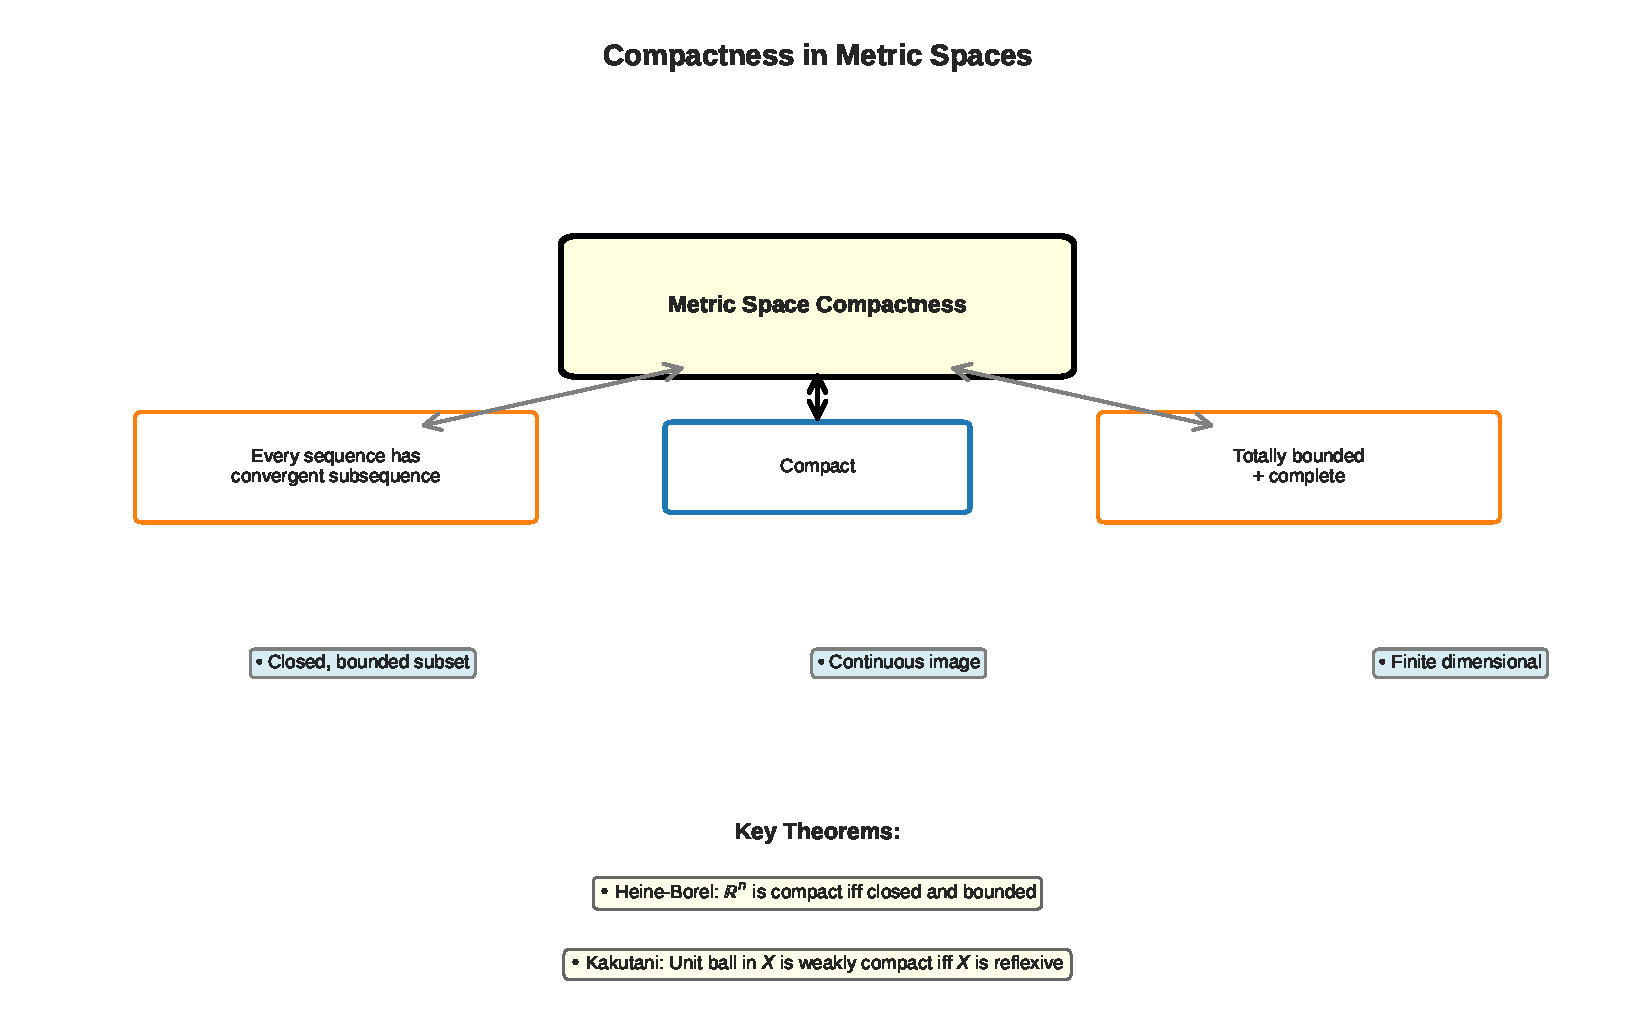
\includegraphics[width=0.65\linewidth]{compactness_relationships.pdf}
  \end{center}
\end{frame}

\begin{frame}{Weak Compactness}
  \begin{definition}[Weakly Compact / Weakly Sequentially Compact]
    \begin{itemize}
      \item $C$ is \textbf{weakly compact} if it is compact in the weak topology
      \item $C$ is \textbf{weakly sequentially compact} if every sequence in $C$ has a weakly convergent subsequence
    \end{itemize}
  \end{definition}

  \vspace{0.3cm}
  \begin{theorem}[Theorem 1.28 --- Eberlein-Šmulian]
    In a Banach space, weak compactness and weak sequential compactness are equivalent.
  \end{theorem}

  \vspace{0.3cm}
  \begin{theorem}[Theorem 1.29 --- Kakutani's Theorem]
    Let $X$ be a Banach space. The closed unit ball $\mathbb{B}_X = \{x : \|x\| \leq 1\}$ is weakly compact iff $X$ is reflexive.
  \end{theorem}

  \vspace{0.3cm}
  \begin{theorem}[Theorem 1.33 --- Banach-Alaoğlu]
    The closed unit ball $\mathbb{B}_{X^*}$ in the dual space $X^*$ is weak* compact.
  \end{theorem}

  \vspace{0.3cm}
  \textbf{Consequence:} Even if unit ball in $X$ is not weakly compact, its dual always has weak* compact unit ball.
\end{frame}

\begin{frame}{Mazur's Theorem and Convexity}
  \begin{theorem}[Theorem 1.27 --- Mazur's Theorem]
    The closed convex hull $\overline{\text{co}}(C)$ of a compact set $C$ in a Banach space is compact.
  \end{theorem}

  \vspace{0.3cm}
  \textbf{Key Lemma:} For reflexive Banach spaces:

  \begin{theorem}[Theorem 1.30]
    A Banach space $X$ is reflexive iff every closed convex bounded subset is weakly compact.
  \end{theorem}

  \vspace{0.3cm}
  \begin{theorem}[Theorem 1.31]
    Let $X$ be a reflexive Banach space and $C \subseteq X$. Then $C$ is weakly compact iff $C$ is bounded (in strong topology).
  \end{theorem}

  \vspace{0.3cm}
  \begin{observation}
    \begin{enumerate}
      \item Strong convergence $\Rightarrow$ weak convergence
      \item Weak convergence $\Rightarrow$ boundedness
      \item Reflexive $\Rightarrow$ weakly complete (weak Cauchy sequences converge)
      \item Closed convex set is weakly closed
    \end{enumerate}
  \end{observation}
\end{frame}

\begin{frame}{Characterization of Reflexivity}
  \begin{theorem}[Theorem 1.32]
    For a Banach space $X$, the following are equivalent:
    \begin{enumerate}
      \item $X$ is reflexive
      \item $\mathbb{B}_X$ is weakly compact
      \item Every bounded sequence has a weakly convergent subsequence
      \item $X^*$ is reflexive
      \item For any $f \in X^*$, there exists $x \in \mathbb{B}_X$ such that $f(x) = \|f\|_*$
      \item Every closed convex bounded subset of $X$ is weakly compact
      \item $\sigma(X^*, X) = \sigma(X^*, X^{**})$ (weak and weak* topologies on $X^*$ coincide)
    \end{enumerate}
  \end{theorem}

  \vspace{0.3cm}
  \textbf{Summary Table:}
  \begin{center}
    \begin{tabular}{|c|c|c|}
      \hline
      \textbf{Space} & \textbf{Reflexive?} & \textbf{Remarks} \\
      \hline
      $\ell^p$ ($1 < p < \infty$) & Yes & Hilbert when $p=2$ \\
      $\ell^1, \ell^\infty$ & No & Dual pairs \\
      $c_0$ & No & Dual is $\ell^1$ \\
      $C[a,b]$ & No & Dual is Radon measures \\
      Hilbert spaces & Yes & All reflexive \\
      \hline
    \end{tabular}
  \end{center}
\end{frame}

\begin{frame}{Summary and Key Takeaways}
  \textbf{Chapter 1b Main Topics:}

  \vspace{0.2cm}
  \begin{enumerate}
    \item \textbf{Linear Operators}: Definition, boundedness, continuity equivalence

    \item \textbf{Hahn-Banach Theorem}: Extends functionals with norm preservation

    \item \textbf{Dual Spaces}: $X^*$, operator norms, duality pairings

    \item \textbf{Weak Topologies}: Weaker than norm topology, useful convergence notion

    \item \textbf{Reflexivity}: When $X = X^{**}$, relates to weak compactness

    \item \textbf{Compactness}: Different in finite vs infinite dimensions
  \end{enumerate}

  \vspace{0.3cm}
  \textbf{Essential Definitions:}
  \begin{itemize}
    \item Banach algebra, reflexive space, weak convergence, Schur property
    \item Natural embedding, dual space, operator norm, sublinear functional
  \end{itemize}

  \vspace{0.3cm}
  \textbf{Most Important Theorems:}
  \begin{itemize}
    \item Hahn-Banach (existence of extending functionals)
    \item Banach-Alaoğlu (weak* compactness of unit ball)
    \item Kakutani-Smulian (reflexivity and weak compactness)
    \item Riesz representation (Hilbert space duality)
  \end{itemize}

  \begin{center}
    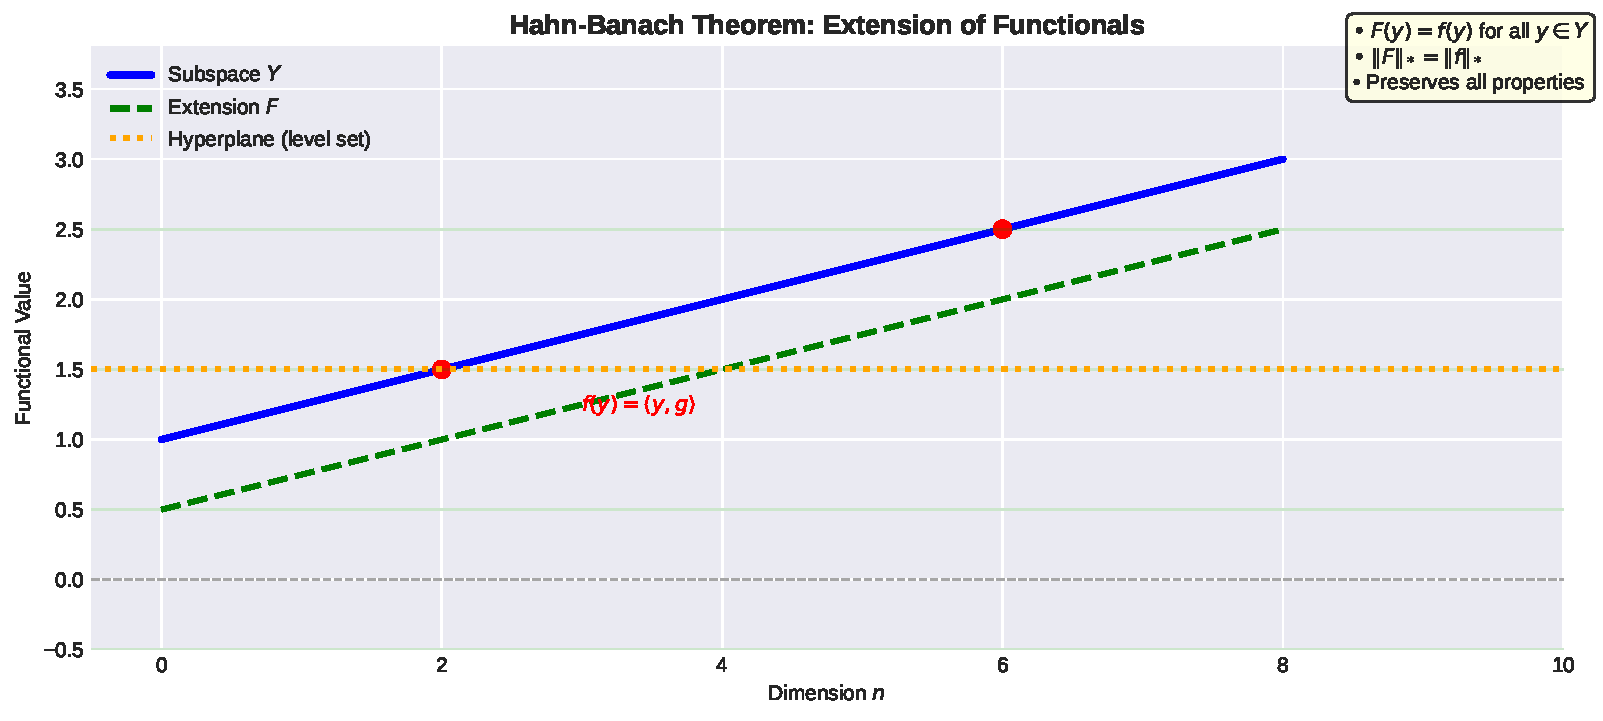
\includegraphics[width=0.5\linewidth]{hahn_banach.pdf}
  \end{center}
\end{frame}

\begin{frame}{Further Reading and Applications}
  \textbf{Next Topics (Chapter 1c onwards):}
  \begin{itemize}
    \item Optimization with weak topologies
    \item Fixed point theorems using compactness
    \item Existence of solutions using Hahn-Banach
  \end{itemize}

  \vspace{0.3cm}
  \textbf{Applications of Hahn-Banach:}
  \begin{itemize}
    \item Separation of convex sets
    \item Characterization of elements by functionals
    \item Extension of linear constraints
    \item Minimax theorems
  \end{itemize}

  \vspace{0.3cm}
  \textbf{Practical Considerations:}
  \begin{itemize}
    \item In finite dimensions: all notions collapse (Heine-Borel, reflexivity automatic)
    \item In infinite dimensions: weak topology essential (fixed points, variational problems)
    \item Computational: weak convergence harder to verify but weaker assumption
  \end{itemize}

  \vspace{0.3cm}
  \begin{center}
    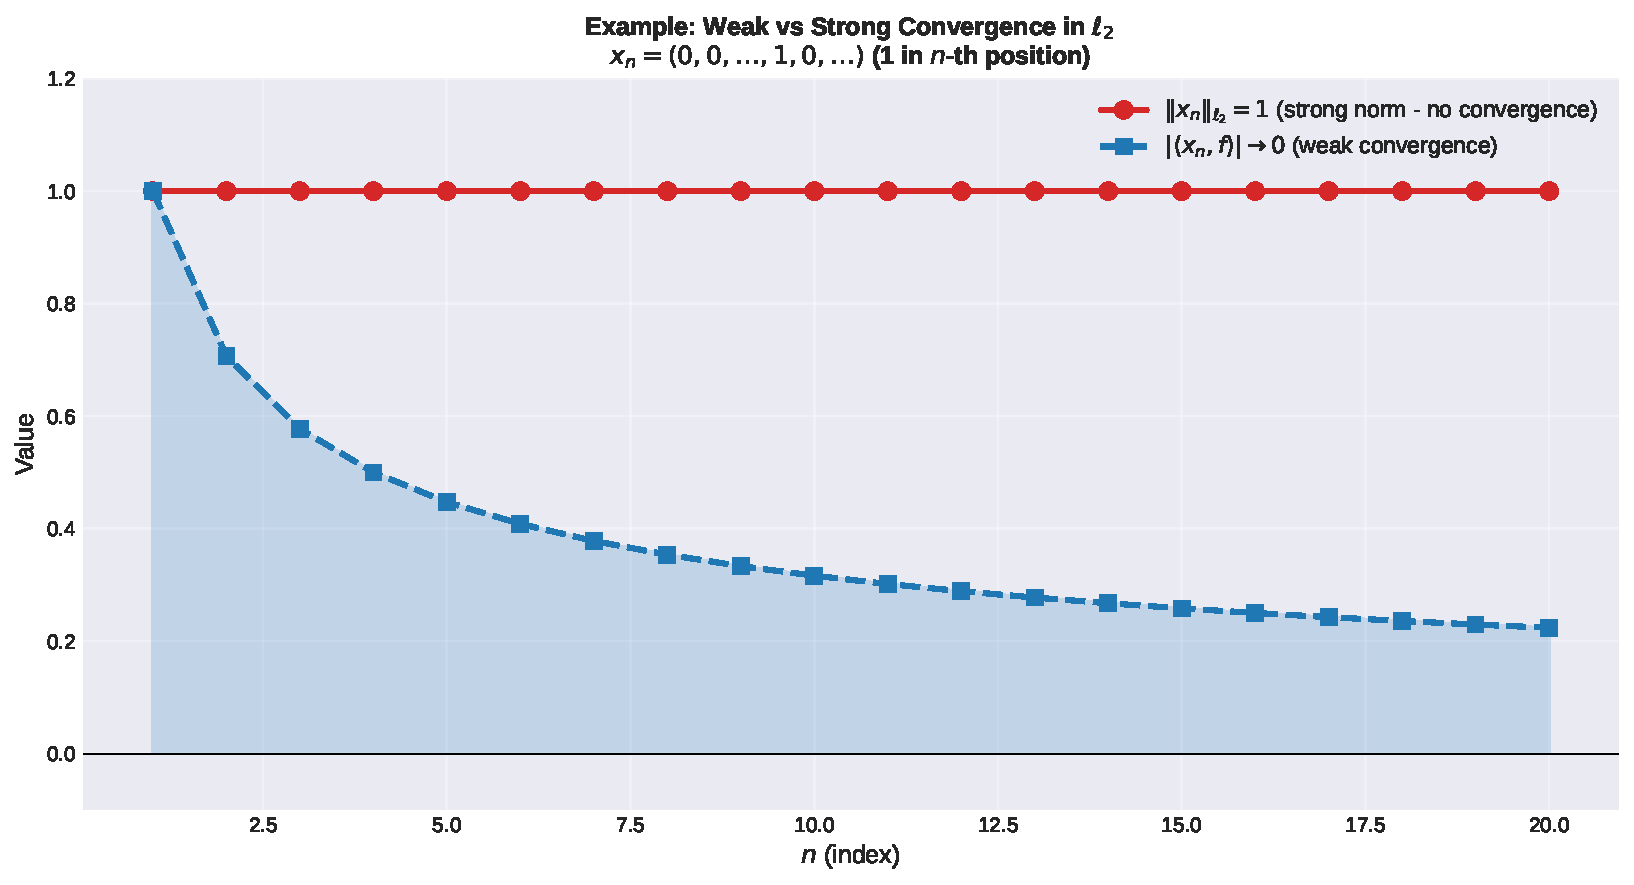
\includegraphics[width=0.5\linewidth]{weak_convergence_example.pdf}
  \end{center}
\end{frame}

\end{document}
